\documentclass{beamer}
% use this instead for 16:9 aspect ratio:
%\documentclass[aspectratio=169]{beamer}
\usepackage{etex}
\usepackage{verbatim}
\reserveinserts{28}
\usetheme{ETHbeamer}

\colorlet{ETHcolor1}{ETHc}
\colorlet{ETHcolor2}{ETHc}

\author{Benjamin Ellenberger}
\institute{INI:  Institute of Neuroinformatics}

\title{How Evolution \_might\_ make creatures walk\\ A multistage optimization problem}

\date{2015-05-13}

%%TODO: Add todo feature
%%TODO: Optimize with presentation tips

% uncomment if you do not want to use a department logo
%\deplogofalse


\begin{document}

\titleframe

\section{A box of candy}

%\begin{frame}

%  \frametitle{Contents}
%  \tableofcontents[currentsection]
%\end{frame}

% Are we alone in the universe?
\begin{minimalframe}
	\hspace*{-1.1cm}
	\vspace*{3cm}
	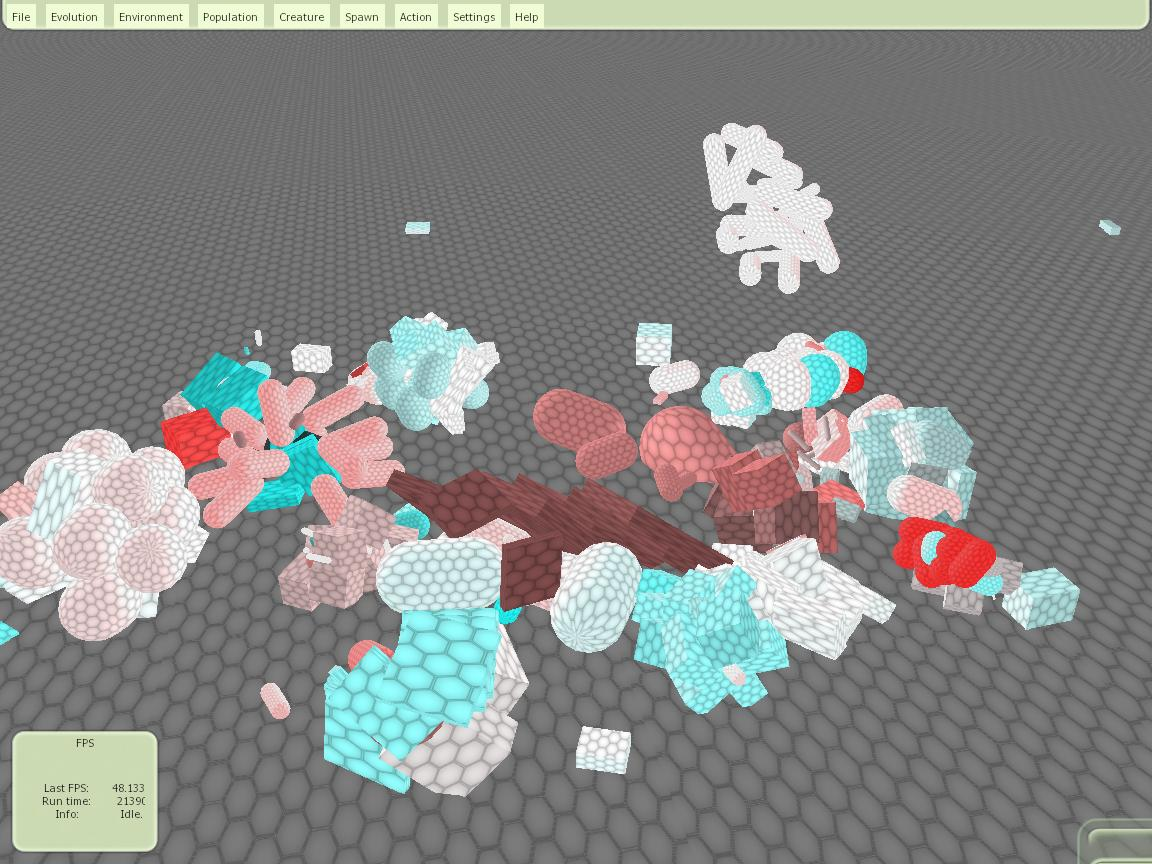
\includegraphics[width=1.2\textwidth,clip]{figs/creatures/Minemonics-05112015_190947481.jpg}
	
\end{minimalframe}

\section{How does evolution optimize?}

\frame{

  \frametitle{How does evolution optimize?}
  
  \begin{columns}
   \column{0.7\textwidth}
 \begin{itemize}
  	\visible<2->{
	     \item Variation-Selection-Replication cycle
	}
	
	\visible<3->{
    	\item Indirect, developmental, messy encoding (redundant, prone to sudden variation)
    	}
	
	\visible<4->{
    	\item Embryogenesis/ Genotype (DNA) to Phenotype (Animal body) transcription
    	}
    	
 	\visible<5->{
    	\item Development of animal after birth (Metamorphosis/ Growth etc.)
 	}
 	
 	\visible<6->{
    	\item Learn to adapt
 	}
 	
 	\visible<6->{
    	\item Nature vs. nurture debate
 	}
     \end{itemize}
     
     \column{0.35\textwidth}
      \visible<1->{
      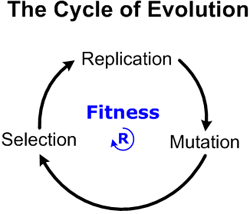
\includegraphics[width=1.5in, clip] {figs/CycleOfEvolution.png} 
      }
  \end{columns}
  }
\note{}

\section{Can we do similar things?}

\frame{

  \frametitle{Contents}
    \tableofcontents[currentsection]
}
\note{}

\subsection{Evolution}

\frame{

  \frametitle{Evolving Virtual Creatures}
  
  \begin{columns}
   \column{0.5\textwidth}
 \begin{itemize}
  	\visible<2->{
	     \item Creatures are built from 3D Primitives and Joints
	}
	
	\visible<3->{
    	\item Sensors, Controller and Effectors make it move
    	}
    	
 	\visible<4->{
    	\item Body and controller co-evolved
 	}
     \end{itemize}
     
     \column{0.5\textwidth}
      \visible<1->{
      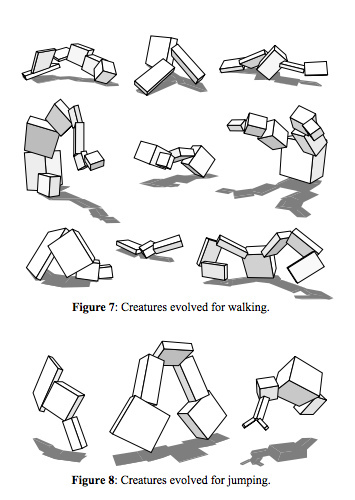
\includegraphics[width=2in, clip] {figs/creatures.jpg} 
      }
  \end{columns}
      \footnotetext[1]{Image from Sims K. - Evolving Virtual Creatures (1994)}
  }
\note{}

\subsection{Genetic language}
\frame{

  \frametitle{Genetic language: Genotype}

\begin{tikzpicture}
   \foreach \c/\i/\t [count=\n] in  
        {blue!20/RootLimb/2,green!20/Limb1/1,orange!20/Limb2/0.8,red!20/Limb3/0.5} 
           \node[draw,fill=\c,minimum height=\t * 1.5cm,minimum width = \t * 1cm,xshift=\n* 2cm](N\n){\i} ;
\draw[dashed,->,line width=0.5mm] (N1.south) to [out=-50,in=-150] node[below] {Branch/2} (N2.south);
\draw[dashed,->,line width=0.5mm] (N2.north) to [out=50,in=150] node[above] {Branch/2} (N3.north);
\draw[dashed,->,line width=0.5mm] (N2.south) to [out=-50,in=-150] node[below] {Branch/2} (N4.south);

\end{tikzpicture}

  \begin{itemize}
\item \textbf{Limb} Part of creature body
\end{itemize}

  
  }
\note{}

\frame{
 \frametitle{Genetic language: Phenotype}

% Set the overall layout of the tree
\tikzstyle{level 1}=[level distance=1cm, sibling distance=6cm]
\tikzstyle{level 2}=[level distance=1.5cm, sibling distance=1.4cm]

% Define styles
\tikzstyle{rl}=[draw,fill=blue!20,minimum height=3cm,minimum width=2cm]
\tikzstyle{l1}=[draw,fill=green!20,minimum height=1.5cm,minimum width=1cm]
\tikzstyle{l2}=[draw,fill=orange!20,minimum height=1.2cm,minimum width=0.8cm]
\tikzstyle{l3}=[draw,fill=red!20,minimum height=0.75cm,minimum width=0.5cm]

\begin{tikzpicture}[grow=down, sloped]
\node[rl] {RootLimb}
    child {
            node[l1] {Limb1}
            child {
                node[l2] {Limb2}
            }
            child {
                node[l3] {Limb3}
            }    
            child {
                node[l3] {Limb3}
            }
            child {
                node[l2] {Limb2}
            }
    }
    child {
            node[l1] {Limb1}
            child {
                node[l2] {Limb2}
            }
            child {
                node[l3] {Limb3}
            }    
            child {
                node[l3] {Limb3}
            }
            child {
                node[l2] {Limb2}
            }
    };
\end{tikzpicture}
  }
\note{}

\frame{

  \frametitle{Genetic language: Phenotype cont.}
  \begin{center}
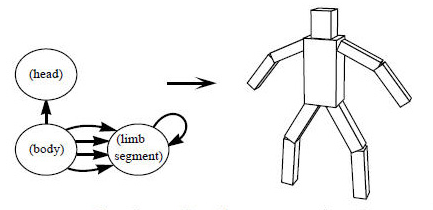
\includegraphics[width=0.8\textwidth, clip] {figs/Sims_Evolve.png}
  \end{center}
    \footnotetext[1]{Image from Sims K. - Evolving Virtual Creatures (1994)}
  }
\note{}

\frame{

  \frametitle{Execution of creatures}
  \begin{columns}
  \column{0.45\textwidth}
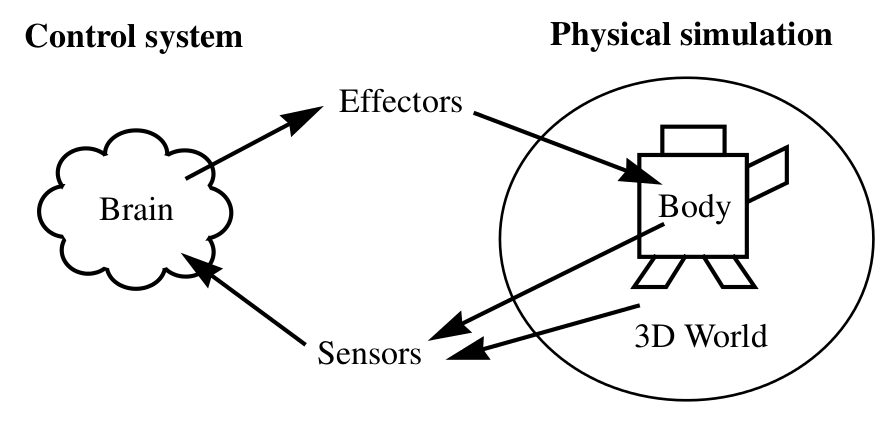
\includegraphics[width=1\textwidth, clip] {figs/brain-body-cycle.png}
 \column{0.55\textwidth}
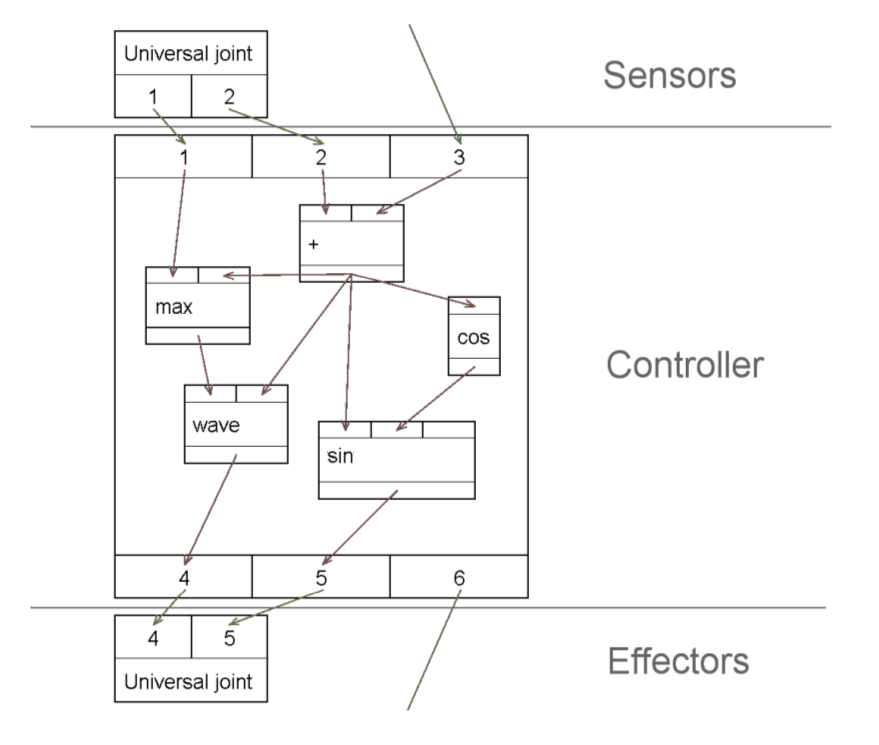
\includegraphics[width=1\textwidth, clip] {figs/execution.png} 
  \end{columns}
  \footnotetext[1]{Image from Sims K. - Evolving Virtual Creatures (1994)}
  }
\note{}

\subsection{Evolution}
\frame{

  \frametitle{Evolution}

\begin{itemize}
\item Selection: Only a certain percentage of creatures are selected for new generation
\item Cross-over: Only certain percentage of creatures are allowed to breed
\item Mutation
\begin{itemize}
\item Other creatures are subject to mutation
\item Mutation of gene
\item Mutation of gene attributes
\item Mutation of gene branches
\end{itemize}
\item Successful creatures stay in the population and the population is refilled with newly bred and mutated ones
\end{itemize}
  
  }
\note{}

\section{Demonstration and Results}

\frame{

  \frametitle{Contents}
    \tableofcontents[currentsection]
}
\note{}

\section{Experiments}
\frame{

  \frametitle{Contents}
    \tableofcontents[currentsection]
}
\note{}

\subsection{Oscillator controller}
\frame{

  \frametitle{Oscillator controller}
  \begin{columns}
  \column{0.6\textwidth}
  \begin{itemize}
  \item Sine-wave controller taking frequency, amplitude, X-shift,Y-shift as input which are determined evolutionarily.
  \end{itemize}
  \column{0.4\textwidth}
  
\includegraphics[width=1.8in, clip] {figs/osc-symbol.png}
  \end{columns}
}
\note{}

\subsubsection{Kuramoto model}

\frame{

  \frametitle{Kuramoto model}
  \begin{columns}
  \column{0.8\textwidth}
  \begin{itemize}
  \item A model proposed by  Yoshiki Kuramoto\footnotemark~to describe synchronization.
  \item \( \frac{d \theta_i}{d t} = \omega_i + \frac{K}{N} \sum\limits_{j=1}^{N} \sin(\theta_j - \theta_i), \qquad i = 1 \ldots N\)
  \end{itemize}
  \column{0.2\textwidth}
  \href{run:./KuramotoModelPhaseLocking.ogv}{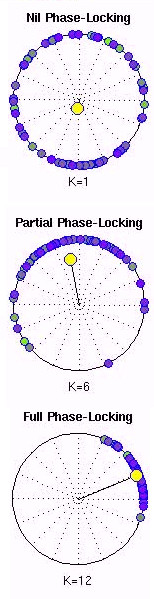
\includegraphics[width=0.6in, clip]{figs/KuramotoModelPhaseLocking-crop.jpg}}
  \end{columns}
  
  \footnotetext[1]{Kuramoto Y. (1984). Chemical Oscillations, Waves, and Turbulence. New York, NY: Springer-Verlag}
}
\note{}



%\subsubsection{Central Pattern Generators}
\subsubsection{Simple limiters theory}

% Simple limiter theory
\begin{frame}
	\frametitle{Simplifying control using simple limiters\footnotemark}
	  \begin{columns}
   \column{0.5\textwidth}
 \begin{itemize}
 	 \visible<1->{
	    \item Generally the chaos controller is more complex than the system it controls
	 }
	 \visible<2>{
    		\item Not true for the simple limiter
    	}

    	\visible<1->{
    	\vspace*{2.9em}
    	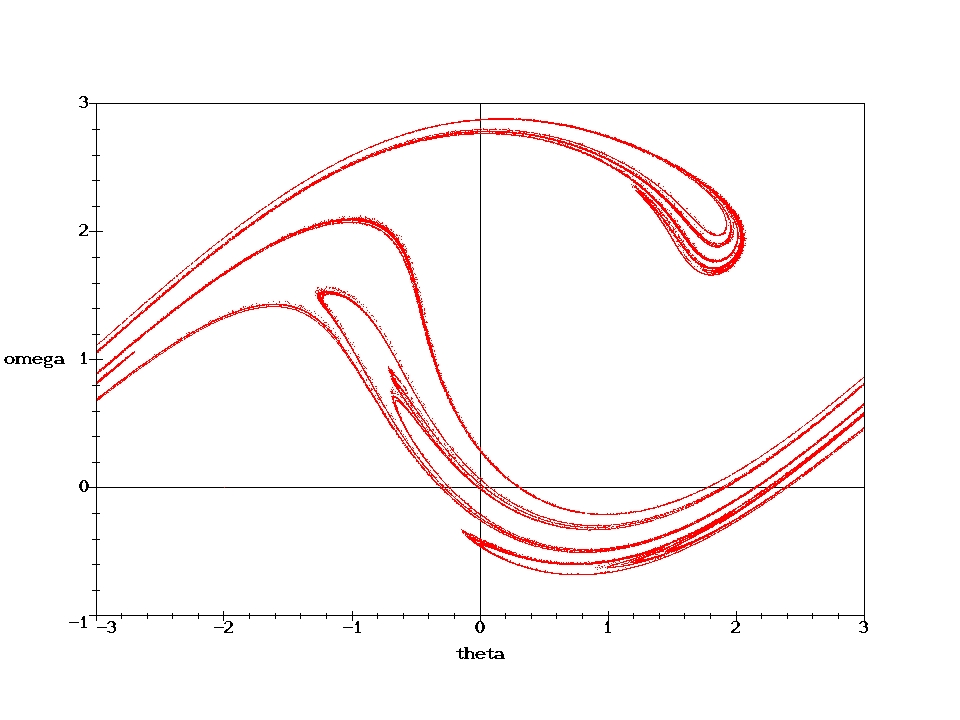
\includegraphics[width=1.7in, clip] {figs/chaotic-driven-pendulum-pcmap.jpeg}
    	}
     \end{itemize}
     \visible<1->{
     \column{0.5\textwidth}
      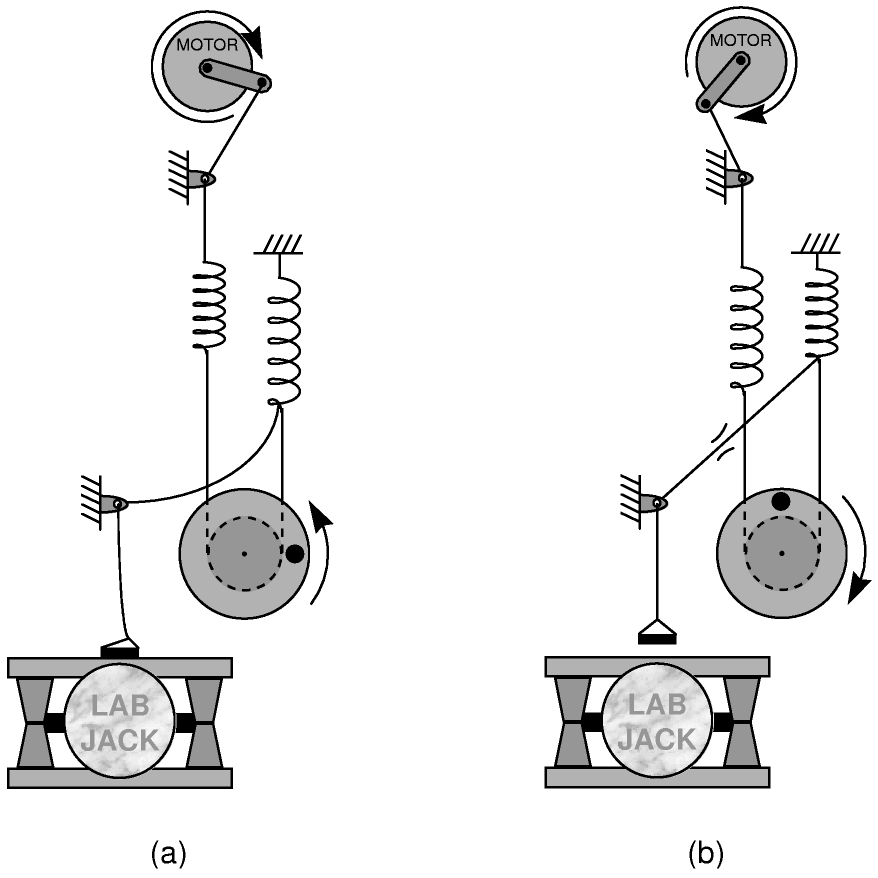
\includegraphics[width=1.4in, clip] {figs/chaotic-driven-pendulum.png}\\
      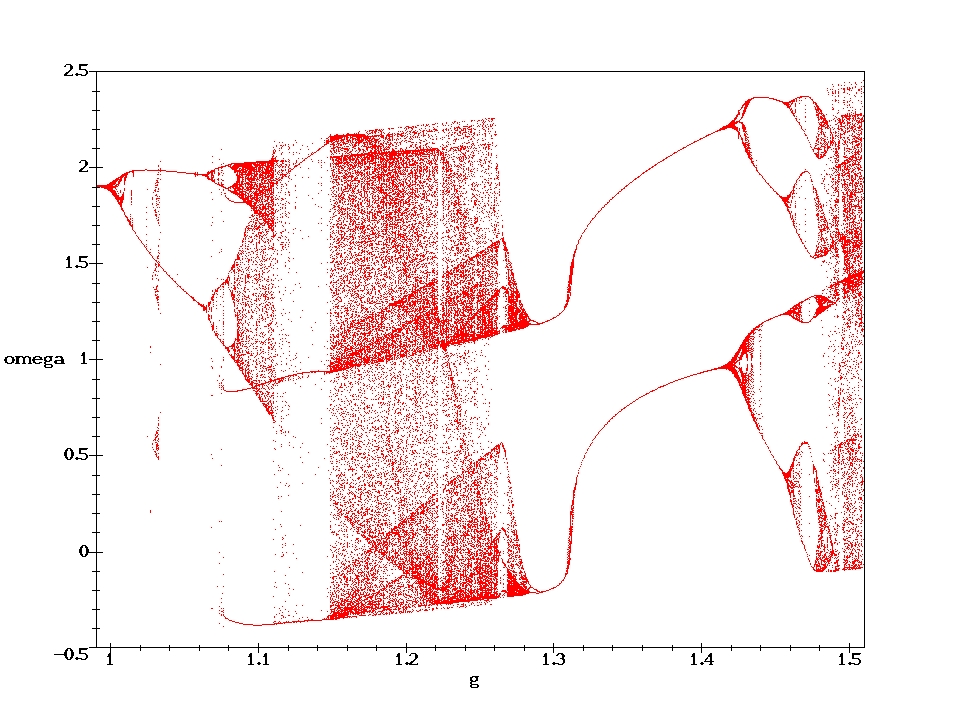
\includegraphics[width=1.55in, clip] {figs/chaotic-driven-pendulum-bifurcationmap.jpeg}
      }
  \end{columns}
  \footnotetext[2]{Corron N. et al. - Controlling Chaos with Simple Limiters (2000)}
\end{frame}

%% Types of simple limiters in nature
\begin{frame}
	\frametitle{Simple limiters in nature}
	\begin{columns}
	\column{.6\textwidth}
	\begin{itemize}
	\visible<2->{
	\item Muscle length \& joint limits
	}
	
	\visible<3->{
	\item The weight of the limbs
	}
	
	\visible<4->{
	\item The relative position of limbs connected by joints\\ (Direction of force applied to joints)
	}
	
	\visible<5>{
	\item The fact that physical objects can not interpenetrate each other
	}
	
	\end{itemize}
\column{.45\textwidth}
     \visible<1->{
		%http://jonbarron.org/article/physiology-muscles
	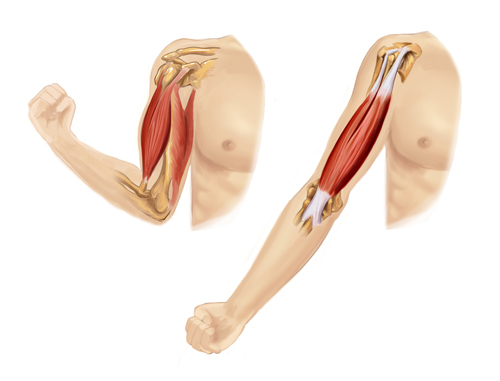
\includegraphics[width=1\textwidth]{figs/natural-limiter-arm-muscle.jpg}
	}
  \end{columns}
\end{frame}

%% Will simple limiters be used if they do not need to be used
\begin{frame}
	\frametitle{In silico\footnote{In silico = in simulation}: Will the simple limiters be used?}
	\begin{columns}
	\column{0.6\textwidth}
	\begin{itemize}
	\visible<2->{
	\item Hypothesis 1: Simple limiters are an omnipresent feature used to reduce the control complexity and to control chaotic movement
	}
	\visible<3->{
	\item Hypothesis 2: If the world is flat then less simple limiters are used, if the world is dynamic and bumpy then more simple limiters are used.
	}
	\visible<4->{
	\item Question remains: Can you live limitless?
	}
	\end{itemize}
	\column{0.5\textwidth}
	\visible<1->{
	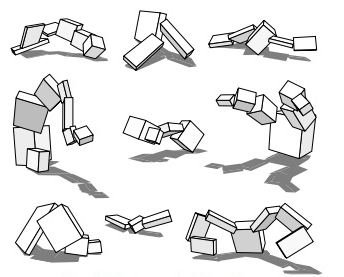
\includegraphics[width=0.8\textwidth]{figs/Sims.png}\\
	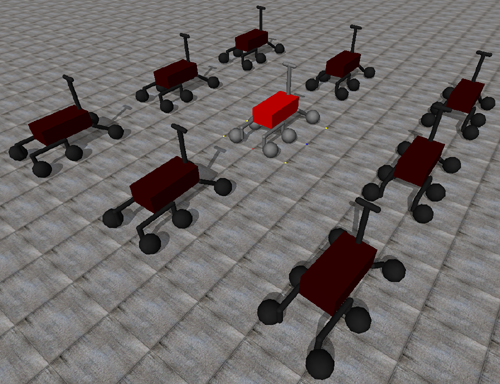
\includegraphics[width=0.8\textwidth]{figs/MarsMadness.png}
	}
	\end{columns}
\end{frame}

\subsection{Reinforcement Learning and Neural network controller}
\frame{

  \frametitle{Reinforcement Learning and Neural network controller}
  \begin{columns}
  \column{0.65\textwidth}
  \begin{itemize}
	\item Reinforcement learning\footnotemark~to make a particular creature learn how to walk
	\item Actor \& Critic Architecture of two Neural Networks
  \end{itemize}
  \column{0.35\textwidth}
  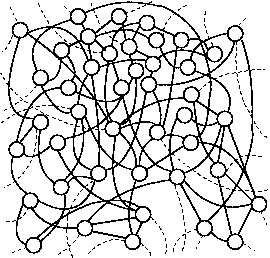
\includegraphics[width=1.5in, clip] {figs/NN.png} 
  \end{columns}
  \footnotetext[3]{Sutton, R. \& Barto, A. Reinforcement Learning: An Introduction (MIT Press, 1998)}
}
\note{}

\frame{

  \frametitle{Google Deepmind \footnotemark: Reinforcement Learning on Atari Games}
  \begin{columns}
  \column{0.6\textwidth}
  \begin{itemize}
	\item can learn successful play policies directly from high-dimensional sensory inputs using end-to-end reinforcement learning
	\item Only for discrete set of actions
  \end{itemize}
  \column{0.4\textwidth}
  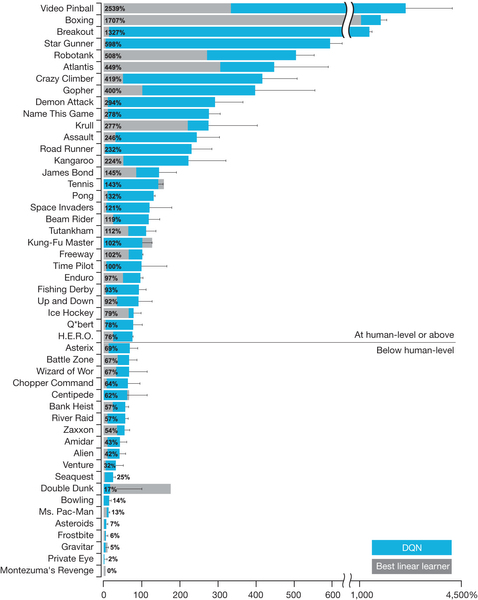
\includegraphics[width=1.8in, clip] {figs/Deep-reinforcement-learning1.jpg} 
  \end{columns}
  \footnotetext[4]{V. Mnih et al., Human-level control through deep reinforcement learning, Nature 518, 529--533 (26 February 2015)}
}
\note{}

\frame{

  \frametitle{Google Deepmind \footnotemark: Continuous control with deep reinforcement learning}
  \begin{columns}
  \column{0.55\textwidth}
  \begin{itemize}
	\item can learn successful policies directly from high-dimensional sensory inputs using end-to-end reinforcement learning
	\item can solve problems such as cartpole swing-up, dexterous manipulation, legged locomotion
	\item actor-critic algorithm that can operate over continuous action spaces
	\vspace{0.5em}
  \end{itemize}
  \column{0.45\textwidth}
  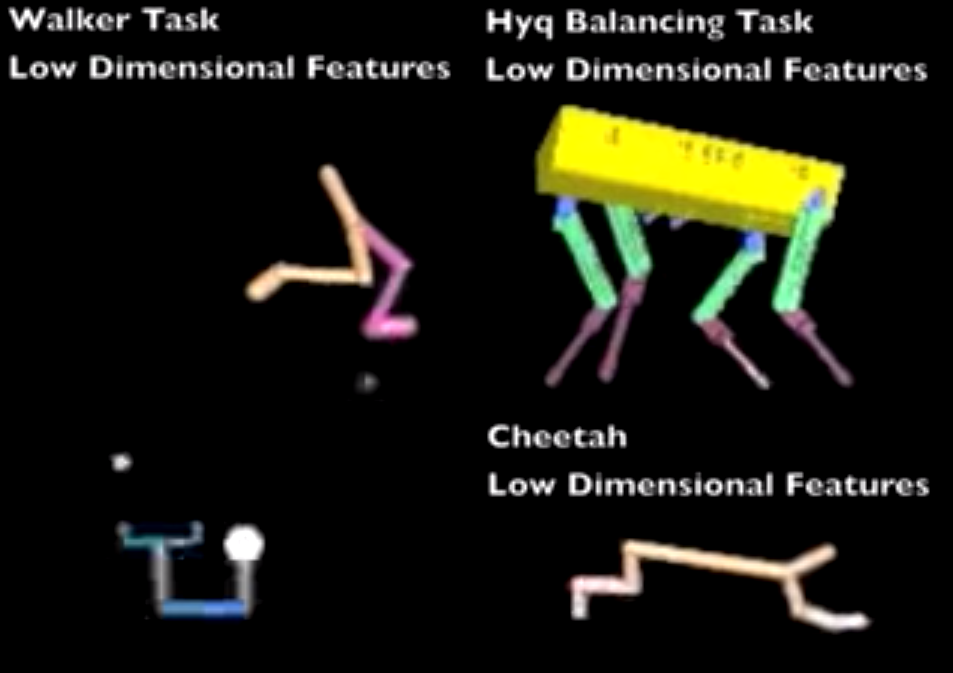
\includegraphics[width=2in, clip] {figs/Continuous-control1.png} 
  \end{columns}
  \footnotetext[4]{T.P. Lillicrap et al., Continuous control with deep reinforcement learning, http://arxiv.org/abs/1509.02971 Stat. ML. (9 Sep 2015)}
}
\note{}

\begin{frame}
\newcommand{\quadrat}{(0,0mm)--(0mm,5mm)--(5mm,5mm)--(5mm,0mm)--(0mm,0mm);}
\begin{center}
	\hspace{-8mm}
	\begin{tikzpicture}[overlay]
		{\draw[ETHa,fill=ETHa] \quadrat}\label{ETH1}
	\end{tikzpicture}
	\hspace{10mm}
	\begin{tikzpicture}[overlay]
		{\draw[ETHb,fill=ETHb]\quadrat}\label{ETH2}
	\end{tikzpicture}
	\hspace{10mm}
	\begin{tikzpicture}[overlay]
		{\draw[ETHc,fill=ETHc]\quadrat}\label{ETH3}
	\end{tikzpicture}
	\hspace{10mm}
	\begin{tikzpicture}[overlay]
		{\draw[ETHd,fill=ETHd] \quadrat}\label{ETH4}
	\end{tikzpicture}
	\hspace{10mm}
	\begin{tikzpicture}[overlay]
		{\draw[ETHe,fill=ETHe] \quadrat}\label{ETH5}
	\end{tikzpicture}
	\hspace{10mm}
	\begin{tikzpicture}[overlay]
		{\draw[ETHf,fill=ETHf] \quadrat}\label{ETH6}
	\end{tikzpicture}
	\hspace{10mm}
	\begin{tikzpicture}[overlay]
		{\draw[ETHg,fill=ETHg] \quadrat}\label{ETH7}
	\end{tikzpicture}
	\hspace{10mm}
	\begin{tikzpicture}[overlay]
		{\draw[ETHh,fill=ETHh] \quadrat}\label{ETH8}
	\end{tikzpicture}
	\hspace{10mm}
	\begin{tikzpicture}[overlay]
		{\draw[ETHi,fill=ETHi] \quadrat}\label{ETH9}
	\end{tikzpicture}\\
	\vspace*{1em}
	{\Huge \textbf{Discussion!}}
\end{center}
\vspace*{1.5em}

\begin{itemize}
\item Any questions?
\item What experiments do you have in mind?
\item What else would you change, extend, enhance, improve etc.?
\item If you have any ideas later, email me: be.ellenberger@gmail.com
\item You can look at my progress: https://github.com/benelot/minemonics
\end{itemize}

\end{frame}


\frame{

  \frametitle{References}
  \begin{itemize}
  \item Sims K. - Evolving Virtual Creatures (1994)
  \item Sims K. - Evolving 3D Morphology and Behavior by Competition (1994)
  \item Krcah P. - Evolving Virtual Creatures Revisited (2007)
  \item Corron N. et al. - Controlling Chaos with Simple Limiters (2000)
  \item Schmidt N. - Bootstrapping perception using information theory: case studies in a quadruped running robot running on different grounds (2013)
  \item Stoop R. - Theory and Simulation of Neural Networks (2014)
  \end{itemize}
}
\note{}

\begin{comment}

% Example slides
\begin{frame}
\textbf{Some mathematical specialities}

\ETHbox{0.8\textwidth}{% define the ETHbox
  \begin{theorem}[Murphy (1949)]\label{murphy}
    Anything that can go wrong, will go wrong.
  \end{theorem}
}

\begin{proof}
  A special case of Theorem \ref{murphy} is proven in %\citet{matthews1995}.
\end{proof}
\end{frame}

\begin{titlestyleframe}
\frametitle{Title Page}

\color{white} The title page is created using the \texttt{\textbackslash titleframe} command.

The title page background can also be used on other frames (or for a customised title frame) using the \texttt{titlestyleframe} environment.
\end{titlestyleframe}

\begin{frame}
\frametitle{Normal Frame}
The normal frame looks like this. It is created using the \texttt{frame} environment.
\end{frame}
\begin{inverseframe}
  \frametitle{Inverse Slides}
  %\color{white}
The inverted frame looks like this. It is created using the \texttt{inverseframe} environment.

 
\end{inverseframe}

\begin{minimalframe}
  \frametitle{Minimal Frame}
The minimal frame looks like this. It is created using the \texttt{minimalframe} environment.
  
\end{minimalframe}

\end{comment}

\end{document}
